\documentclass{beamer}
\usepackage[utf8]{inputenc}
\usepackage{graphicx, epsfig}
\usepackage{amsmath,mathrsfs,amsfonts,amssymb}
\usepackage{floatflt}
\usepackage{epic,ecltree}
\usepackage{mathtext}
\usepackage{fancybox}
\usepackage{fancyhdr}
\usepackage{multirow}
\usepackage{enumerate}
\usepackage{epstopdf}
\usepackage{multicol}
\usepackage{algorithm}
\usepackage[noend]{algorithmic}
\usepackage{tikz}
\usepackage{blindtext}
\usetheme{default}%{Singapore}%{Warsaw}%{Warsaw}%{Darmstadt}
\usecolortheme{default}

\setbeamerfont{title}{size=\Huge}
\setbeamertemplate{footline}[page number]{}

\setbeamertemplate{section in toc}[sections numbered]


\makeatletter
\newcommand\HUGE{\@setfontsize\Huge{35}{40}}
\makeatother    

\setbeamerfont{title}{size=\HUGE}
\beamertemplatenavigationsymbolsempty

% latin bold lower
\newcommand{\ba}{\mathbf{a}} 
\newcommand{\bc}{\mathbf{c}} 
\newcommand{\be}{\mathbf{e}} 
\newcommand{\bh}{\mathbf{h}} 
\newcommand{\bp}{\mathbf{p}} 
\newcommand{\bt}{\mathbf{t}} 
\newcommand{\bs}{\mathbf{s}} 
\newcommand{\bu}{\mathbf{u}} 
\newcommand{\bv}{\mathbf{v}} 
\newcommand{\bw}{\mathbf{w}} 
\newcommand{\bx}{\mathbf{x}} 
\newcommand{\by}{\mathbf{y}} 
\newcommand{\bz}{\mathbf{z}} 

% latin bold upper
\newcommand{\bA}{\mathbf{A}} 
\newcommand{\bB}{\mathbf{B}} 
\newcommand{\bC}{\mathbf{C}} 
\newcommand{\bI}{\mathbf{I}} 
\newcommand{\bJ}{\mathbf{J}} 
\newcommand{\bL}{\mathbf{L}} 
\newcommand{\bM}{\mathbf{M}} 
\newcommand{\bP}{\mathbf{P}}
\newcommand{\bQ}{\mathbf{Q}} 
\newcommand{\bR}{\mathbf{R}} 
\newcommand{\bT}{\mathbf{T}} 
\newcommand{\bU}{\mathbf{U}} 
\newcommand{\bV}{\mathbf{V}} 
\newcommand{\bW}{\mathbf{W}} 
\newcommand{\bX}{\mathbf{X}} 
\newcommand{\bY}{\mathbf{Y}} 
\newcommand{\bZ}{\mathbf{Z}} 

% latin cal upper
\newcommand{\cF}{\mathcal{F}} 
\newcommand{\cG}{\mathcal{G}} 
\newcommand{\cI}{\mathcal{I}} 
\newcommand{\cL}{\mathcal{L}} 
\newcommand{\cM}{\mathcal{M}} 
\newcommand{\cN}{\mathcal{N}} 
\newcommand{\cS}{\mathcal{S}} 
\newcommand{\cT}{\mathcal{T}} 
\newcommand{\cW}{\mathcal{W}} 
\newcommand{\cX}{\mathcal{X}} 
\newcommand{\cZ}{\mathcal{Z}} 

% latin bb upper
\newcommand{\bbE}{\mathbb{E}} 
\newcommand{\bbI}{\mathbb{I}} 
\newcommand{\bbP}{\mathbb{P}} 
\newcommand{\bbR}{\mathbb{R}} 

% greek bold lower
\newcommand{\bepsilon}{\boldsymbol{\epsilon}} 
\newcommand{\btheta}{\boldsymbol{\theta}} 
\newcommand{\blambda}{\boldsymbol{\lambda}} 
\newcommand{\bpi}{\boldsymbol{\pi}} 
\newcommand{\bmu}{\boldsymbol{\mu}} 
\newcommand{\bsigma}{\boldsymbol{\sigma}} 
\newcommand{\bphi}{\boldsymbol{\phi}} 

% greek bold upper
\newcommand{\bSigma}{\boldsymbol{\Sigma}} 

\DeclareMathOperator*{\argmin}{arg\,min}
\DeclareMathOperator*{\argmax}{arg\,max}

\newcommand{\createdgmtitle}[1]{\title[\hbox to 56mm{Deep Generative Models  \hfill\insertframenumber\,/\,\inserttotalframenumber}]
	{\vspace{1cm} \\ Deep Generative Models \\ {\Huge Lecture #1}}
	\author{Roman Isachenko}
	\institute{
	Moscow Institute of Physics and Technology
	} 
	\date{2023, Autumn}
}

\usepackage{tikz}
\usetikzlibrary{arrows,shapes,positioning,shadows,trees}

\newcommand\myfootnote[1]{%
  \tikz[remember picture,overlay]
  \draw (current page.south west) +(1in + \oddsidemargin,0.5em)
  node[anchor=south west,inner sep=0pt]{\parbox{\textwidth}{%
      \rlap{\rule{10em}{0.4pt}}\raggedright\scriptsize \textit{#1}}};}

\newcommand\myfootnotewithlink[2]{%
  \tikz[remember picture,overlay]
  \draw (current page.south west) +(1in + \oddsidemargin,0.5em)
  node[anchor=south west,inner sep=0pt]{\parbox{\textwidth}{%
      \rlap{\rule{10em}{0.4pt}}\raggedright\scriptsize\href{#1}{\textit{#2}}}};}
      
\AtBeginSection[]
      {
      	\begin{frame}{Outline}
      		\tableofcontents[currentsection]
      	\end{frame}
      }
      \AtBeginSubsection[]{
      	\begin{frame}{Outline}
      		\tableofcontents[currentsection,currentsubsection]
      	\end{frame}
}
\createdgmtitle{9}
%--------------------------------------------------------------------------------
\begin{document}
%--------------------------------------------------------------------------------
\begin{frame}[noframenumbering,plain]
%\thispagestyle{empty}
\titlepage
\end{frame}
%=======
\begin{frame}{Recap of previous lecture}
	\begin{block}{Main problems of standard GAN}
		\begin{itemize}
			\item Vanishing gradients (solution: non-saturating GAN);
			\item Mode collapse (caused by Jensen-Shannon divergence).
		\end{itemize}
	\end{block}
	\begin{block}{Standard GAN}
		\vspace{-0.7cm}
		\[
			\min_{\btheta} \max_{\bphi} \left[ \bbE_{\pi(\bx)} \log D(\bx, \bphi) + \bbE_{p(\bz)} \log (1 - D(G(\bz, \btheta), \bphi)) \right]
		\]
		\vspace{-0.7cm}
	\end{block}
	\vspace{-0.1cm}
	\begin{block}{Informal theoretical results}
		The real images distribution $\pi(\bx)$ and the generated images distribution $p(\bx | \btheta)$ are low-dimensional and have disjoint supports. In this case
		\vspace{-0.3cm}
		\[
			KL(\pi || p) = KL(p || \pi) = \infty, \quad JSD(\pi || p) = \log 2.
		\]
		\end{block}
		\myfootnote{\href{https://arxiv.org/abs/1406.2661}{Goodfellow I. J. et al. Generative Adversarial Networks, 2014} \\
		\href{https://arxiv.org/abs/1701.04862}{Arjovsky M., Bottou L. Towards Principled Methods for Training Generative Adversarial Networks, 2017}}
\end{frame}
%=======
\begin{frame}{Recap of previous lecture}
		\begin{block}{Wasserstein distance}
			\vspace{-0.5cm}
			\[
				W(\pi, p) = \inf_{\gamma \in \Gamma(\pi, p)} \bbE_{(\bx, \by) \sim \gamma} \| \bx - \by \| =  \inf_{\gamma \in \Gamma(\pi, p)} \int \| \bx - \by \| \gamma (\bx, \by) d \bx d \by
			\]
			\vspace{-0.5cm}
			\begin{itemize}
				\item $\gamma(\bx, \by)$ -- transportation plan (the amount of "dirt" that should be transported from point $\bx$ to point $\by$).
				\item $\Gamma(\pi, p)$ -- the set of all joint distributions $\Gamma (\bx, \by)$ with marginals $\pi$ and $p$ ($\int \gamma(\bx, \by) d \bx = p(\by)$, $\int \gamma(\bx, \by) d \by = \pi(\bx)$).
				\item $\gamma(\bx, \by)$ -- the amount, $\|\bx - \by \|$-- the distance.
			\end{itemize}
		\end{block}
		\begin{block}{Theorem (Kantorovich-Rubinstein duality)}
			\vspace{-0.2cm}
			\[
				W(\pi || p) = \frac{1}{K} \max_{\| f \|_L \leq K} \left[ \bbE_{\pi(\bx)} f(\bx)  - \bbE_{p(\bx)} f(\bx)\right],
			\]
			where $\| f \|_L \leq K$ are $K-$Lipschitz continuous functions ($f: \cX \rightarrow \bbR$).
		\end{block}
		\myfootnotewithlink{https://arxiv.org/abs/1701.07875}{Arjovsky M., Chintala S., Bottou L. Wasserstein GAN, 2017}
\end{frame}
%=======
\begin{frame}{Recap of previous lecture}
	\begin{block}{WGAN objective}
		\vspace{-0.5cm}
		\[
		\min_{\btheta} W(\pi || p) = \min_{\btheta} \max_{\bphi \in \boldsymbol{\Phi}} \left[ \bbE_{\pi(\bx)} f(\bx, \bphi)  - \bbE_{p(\bz)} f(G(\bz, \btheta), \bphi )\right].
		\]
		\vspace{-0.5cm}
	\end{block}
	\begin{itemize}
		\item Function~$f$ in WGAN is usually called $\textit{critic}$.
		\item If parameters $\bphi$ lie in a compact set $\boldsymbol{\Phi} \in [-c, c]^d$ then $f(\bx, \bphi)$ will be $K$-Lipschitz continuous function. 
	\end{itemize}
	\begin{multline*}
		K \cdot W(\pi || p) = \max_{\| f \|_L \leq K} \left[ \bbE_{\pi(\bx)} f(\bx)  - \bbE_{p(\bx)} f(\bx)\right] \geq \\  \geq \max_{\bphi \in \boldsymbol{\Phi}} \left[ \bbE_{\pi(\bx)} f(\bx, \bphi)  - \bbE_{p(\bx)} f(\bx, \bphi )\right]
	\end{multline*}
	\textit{"Weight clipping is a clearly terrible way to enforce a Lipschitz constraint"}
	\myfootnotewithlink{https://arxiv.org/abs/1701.07875}{Arjovsky M., Chintala S., Bottou L. Wasserstein GAN, 2017}
\end{frame}
%=======
\begin{frame}{Recap of previous lecture}
	\begin{block}{Theorem}
		Let $\pi(\bx)$ and $p(\bx)$ be two distribution in $\cX$, a compact metric space. Let $\gamma$ be the optimal transportation plan between $\pi(\bx)$ and $p(\bx)$. Then
		\vspace{-0.4cm}
		\[
			\bbP_{(\by, \bz) \sim \gamma} \left[ \nabla f^*(\hat{\bx}_t) = \frac{\bz - \hat{\bx}_t}{\| \bz - \hat{\bx}_t \|} \right] = 1.
		\]
		\vspace{-0.6cm}
	\end{block}
	\begin{block}{Gradient penalty}
		\vspace{-0.5cm}
		\[
			W(\pi || p) = \underbrace{\bbE_{\pi(\bx)} f(\bx)  - \bbE_{p(\bx)} f(\bx)}_{\text{original critic loss}} + \lambda \underbrace{\bbE_{U[0, 1]} \left[ \left( \| \nabla f(\hat{\bx}) \|_2 - 1 \right) ^ 2\right]}_{\text{gradient penalty}}.
		\]
		\vspace{-0.5cm}
	\end{block}
	Samples $\hat{\bx}_t = t \by + (1 - t) \bz$ with $t \in [0, 1]$ are uniformly sampled along straight lines between pairs of points: $\by$ from the data distribution $\pi(\bx)$ and $\bz$ from the generator distribution $p(\bx | \btheta)$.
	\myfootnote{
	\href{https://arxiv.org/abs/1701.07875}{Arjovsky M., Chintala S., Bottou L. Wasserstein GAN, 2017} \\
	\href{https://arxiv.org/abs/1704.00028}{Gulrajani I. et al. Improved Training of Wasserstein GANs, 2017} }
\end{frame}
%=======
\begin{frame}{Recap of previous lecture}
	\vspace{-0.3cm}
	\[
		f(\bx, \bphi) = \bW_{K+1} \sigma_K (\bW_K \sigma_{K-1}(\dots \sigma_1(\bW_1 \bx) \dots)).
	\]
	\vspace{-0.3cm}
	\begin{itemize}
		\item $\sigma_k$ is a pointwise nonlinearities. We assume that $\| \sigma_k \|_L = 1$ (it holds for ReLU).
		\item $\mathbf{g}(\bx) = \bW \bx$ is a linear transformation ($\nabla \mathbf{g}(\bx) = \bW$).
		\[
			\| \mathbf{g} \|_L = \sup_\bx \| \nabla \mathbf{g}(\bx) \|_2 = \|\bW\|_2.
		\]
	\end{itemize}
	\vspace{-0.5cm}
	\begin{block}{Critic spectral norm}
		\vspace{-0.5cm}
		\[
			\| f \|_L \leq \| \bW_{K+1}\|_2 \cdot \prod_{k=1}^K  \| \sigma_k \|_L \cdot \| \bW_k \|_2 = \prod_{k=1}^{K+1} \|\bW_k\|_2.
		\]
		\vspace{-0.5cm}
	\end{block}
	\begin{block}{Spectral Normalization GAN}
	If we replace the weights in the critic $f(\bx, \bphi)$ by $\bW^{SN}_k = \bW_k / \|\bW_k\|_2$, we will get $\| f\|_L \leq 1.$ \\
	\end{block}
	 Power iteration approximates the value of $\|\bW\|_2$.
	\myfootnotewithlink{https://arxiv.org/abs/1802.05957}{Miyato T. et al. Spectral Normalization for Generative Adversarial Networks, 2018}
\end{frame}
%=======
\begin{frame}{Outline}
	\tableofcontents
\end{frame}
%=======
\section{f-divergence minimization}
%=======
\begin{frame}{Divergences}
	\begin{itemize}
		\item Forward KL divergence in maximum likelihood estimation.
		\item Reverse KL in variational inference.
		\item JS divergence in standard GAN.
		\item Wasserstein distance in WGAN.
	\end{itemize}
	\begin{block}{What is a divergence?}
		Let $\cS$ be the set of all possible probability distributions. Then $D: \cS \times \cS \rightarrow \bbR$ is a divergence if 
		\begin{itemize}
			\item $D(\pi || p) \geq 0$ for all $\pi, p \in \cS$;
			\item $D(\pi || p) = 0$ if and only if $\pi \equiv p$.
		\end{itemize}
	\end{block}
	\begin{block}{General divergence minimization task}
		\vspace{-0.3cm}
		\[
			\min_p D(\pi || p)
		\]
		\vspace{-0.7cm}
	\end{block}
	\begin{block}{Chalenge}
		We do not know the real distribution $\pi(\bx)$!
	\end{block}
\end{frame}
%=======
\begin{frame}{f-divergence family}
	
	\begin{block}{f-divergence}
		\vspace{-0.3cm}
		\[
		D_f(\pi || p) = \bbE_{p(\bx)}  f\left( \frac{\pi(\bx)}{p(\bx)} \right)  = \int p(\bx) f\left( \frac{\pi(\bx)}{p(\bx)} \right) d \bx.
		\]
		Here $f: \bbR_+ \rightarrow \bbR$ is a convex, lower semicontinuous function satisfying $f(1) = 0$.
	\end{block}
	\begin{figure}
		\centering
		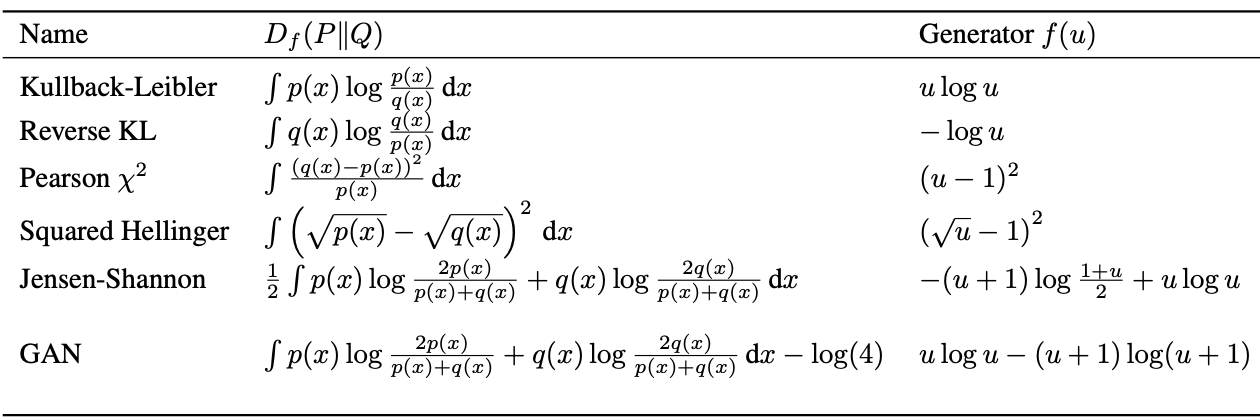
\includegraphics[width=\linewidth]{figs/f_divs}
	\end{figure}
	\myfootnotewithlink{https://arxiv.org/abs/1606.00709}{Nowozin S., Cseke B., Tomioka R. f-GAN: Training Generative Neural Samplers using Variational Divergence Minimization, 2016}
\end{frame}
%=======
\begin{frame}{f-divergence family}
	\vspace{-0.2cm}
	\begin{block}{Fenchel conjugate}
		\vspace{-0.7cm}
		\[
		f^*(t) = \sup_{u \in \text{dom}_f} \left( ut - f(u) \right), \quad f(u) = \sup_{t \in \text{dom}_{f^*}} \left( ut - f^*(t) \right)
		\]
		\vspace{-0.5cm}
	\end{block}
	\textbf{Important property:} $ f^{**} = f$ for convex $f$.
	\begin{block}{f-divergence}
		\vspace{-0.8cm}
		\begin{multline*}
			D_f(\pi || p) = \bbE_{p(\bx)}  f\left( \frac{\pi(\bx)}{p(\bx)} \right)  = \int p(\bx) {\color{violet}f\left( \frac{\pi(\bx)}{p(\bx)} \right) } d \bx = \\ = \int p(\bx) {\color{violet} \sup_{t \in \text{dom}_{f^*}} \left( \frac{\pi(\bx)}{p(\bx)} t - f^*(t) \right)} d \bx = \\ 
			= \int \sup_{t \in \text{dom}_{f^*}} \left( \pi(\bx)t - p(\bx) f^*(t) \right) d \bx .
		\end{multline*}
		\vspace{-0.6cm}
	\end{block}
	Here we seek value of $t$, which gives us maximum value of $ \pi(\bx)t - p(\bx) f^*(t)$, for each data point $\bx$.
	\myfootnotewithlink{https://arxiv.org/abs/1606.00709}{Nowozin S., Cseke B., Tomioka R. f-GAN: Training Generative Neural Samplers using Variational Divergence Minimization, 2016}
\end{frame}
%=======
\begin{frame}{f-divergence family}
	\vspace{-0.4cm}
	\begin{block}{f-divergence}
		\vspace{-0.3cm}
		\[
		D_f(\pi || p) = \bbE_{p(\bx)}  f\left( \frac{\pi(\bx)}{p(\bx)} \right)  = \int p(\bx) f\left( \frac{\pi(\bx)}{p(\bx)} \right) d \bx.
		\]
		\vspace{-0.4cm}
	\end{block}
	\begin{block}{Variational f-divergence estimation}
		\vspace{-0.8cm}
		\begin{multline*}
			D_f(\pi || p)  = {\color{violet}\int} {\color{teal} \sup_{t \in \text{dom}_{f^*}}} \left( \pi(\bx)t - p(\bx) f^*(t) \right) d \bx \geq \\
			 \geq {\color{teal}\sup_{T \in \cT}} {\color{violet}\int} \left( \pi(\bx)T(\bx) - p(\bx) f^*(T(\bx)) \right) d \bx = \\
			 = \sup_{T \in \cT} \left[\bbE_{\pi}T(\bx) -  \bbE_p f^*(T(\bx)) \right]
		\end{multline*}
	\vspace{-0.6cm}
	\end{block}
	This is a lower bound because of Jensen inequality and restricted class of functions $\cT: \cX \rightarrow \bbR$. 
	
	\myfootnotewithlink{https://arxiv.org/abs/1606.00709}{Nowozin S., Cseke B., Tomioka R. f-GAN: Training Generative Neural Samplers using Variational Divergence Minimization, 2016}
\end{frame}
%=======
\begin{frame}{f-divergence family}
	\begin{block}{Variational divergence estimation}
		\[
			D_f(\pi || p) \geq \sup_{T \in \cT} \left[\bbE_{\pi}T(\bx) -  \bbE_p f^*(T(\bx)) \right]
		\]
		The lower bound is tight for $T^*(\bx) = f'\left( \frac{\pi(\bx)}{p(\bx)} \right)$.
	\end{block}
	\begin{block}{Example (JSD)}
		\begin{itemize}
			\item Let define function $f$ and its conjugate $f^*$
			\[ 
				f(u) = u \log u - (u + 1) \log (u + 1), \quad f^*(t) = - \log (1 - e^t).
			\]
			\item Let reparametrize $T(\bx) = \log D(\bx)$.
		\end{itemize}
		\vspace{-0.4cm}
	\end{block}
	\[
		\min_{G} \max_D \left[ \bbE_{\pi(\bx)} \log D(\bx) + \bbE_{p(\bz)} \log (1 - D(G(\bz))) \right]
	\]

	\myfootnotewithlink{https://arxiv.org/abs/1606.00709}{Nowozin S., Cseke B., Tomioka R. f-GAN: Training Generative Neural Samplers using Variational Divergence Minimization, 2016}
\end{frame}
%=======
\begin{frame}{f-divergence family}
	\begin{block}{Variational divergence estimation}
		\[
			D_f(\pi || p) \geq \sup_{T \in \cT} \left[\bbE_{\pi}T(\bx) -  \bbE_p f^*(T(\bx)) \right]
		\]
	\end{block}
	\textbf{Note:} To evaluate lower bound we only need samples from $\pi(\bx)$ and $p(\bx)$. Hence, we could fit implicit generative model.
	\begin{figure}
		\centering
		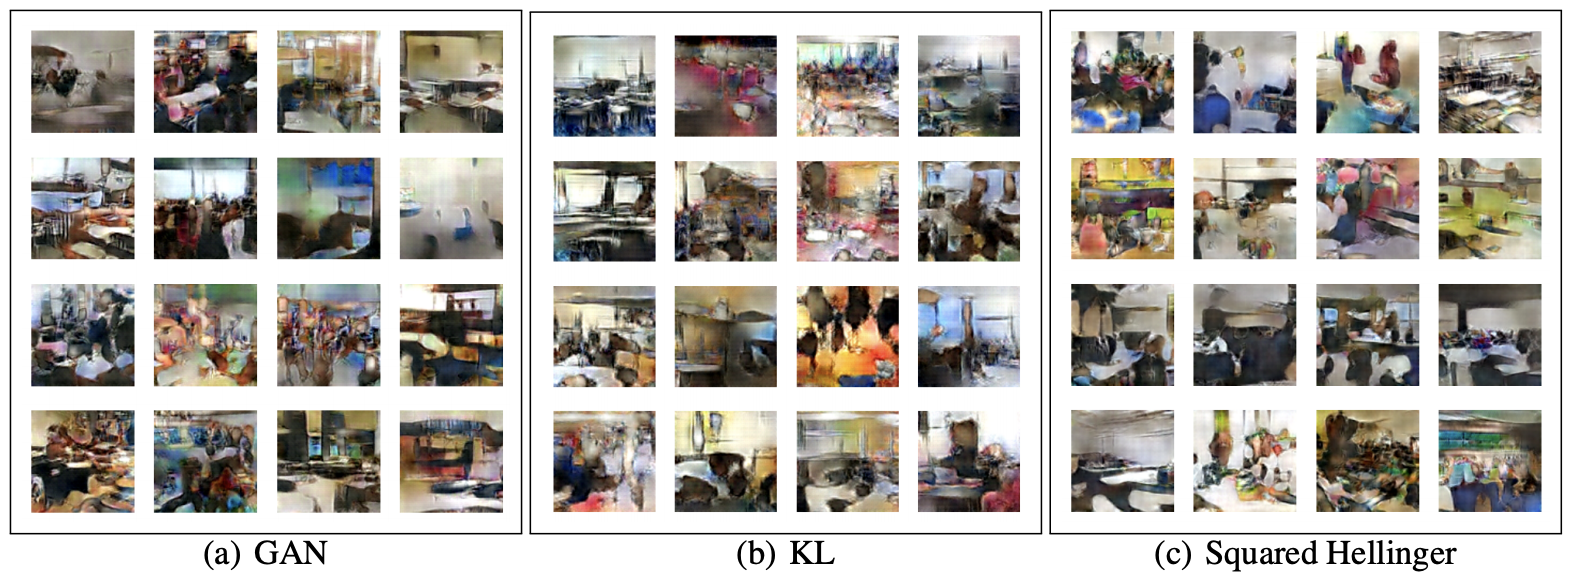
\includegraphics[width=1.0\linewidth]{figs/f_div_results}
	\end{figure}

	\myfootnotewithlink{https://arxiv.org/abs/1606.00709}{Nowozin S., Cseke B., Tomioka R. f-GAN: Training Generative Neural Samplers using Variational Divergence Minimization, 2016}
\end{frame}
%=======
\section{Evaluation of likelihood-free models}
%=======
\begin{frame}{Evaluation of likelihood-free models}
	How to evaluate generative models?
	\begin{block}{Likelihood-based models}
		\begin{itemize}
			\item Split data to train/val/test.
			\item Fit model on the train part.
			\item Tune hyperparameters on the validation part.
			\item Evaluate generalization by reporting likelihoods on the test set.
		\end{itemize}
	\end{block}
	\begin{block}{Not all models have tractable likelihoods}
		\begin{itemize}
			\item VAE: compare ELBO values.
			\item GAN: ???
		\end{itemize}
	\end{block}
\end{frame}
%=======
\begin{frame}{Evaluation of likelihood-free models}
	Let take some pretrained image classification model to get the conditional label distribution $p(y | \bx)$ (e.g. ImageNet classifier).
	\begin{block}{What do we want from samples?}
		\begin{itemize}
			\item \textbf{Sharpness}
			\begin{figure}
				\centering
				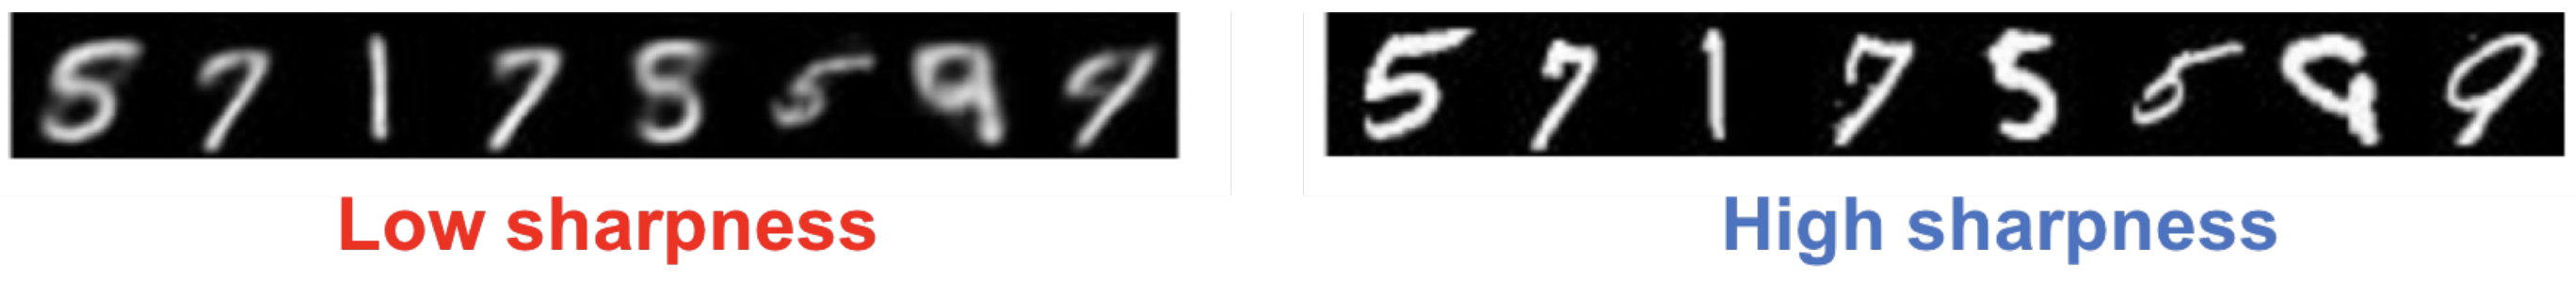
\includegraphics[width=0.9\linewidth]{figs/sharpness}
			\end{figure}
			The conditional distribution $p(y | \bx)$ should have low entropy (each image $\bx$ should have distinctly recognizable object).
			\item \textbf{Diversity}
			\begin{figure}
				\centering
				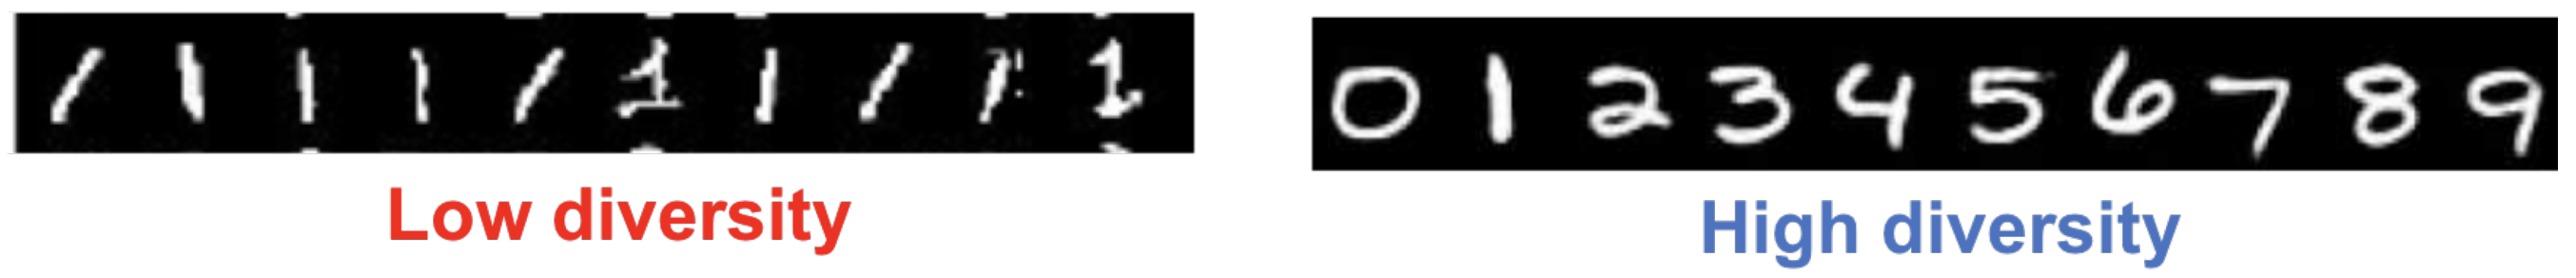
\includegraphics[width=0.9\linewidth]{figs/diversity}
			\end{figure}
			The marginal distribution $p(y) = \int p(y | \bx) p(\bx) d \bx$ should have high entropy (there should be as many classes generated as possible).
		\end{itemize}
	\end{block}
	\myfootnotewithlink{https://deepgenerativemodels.github.io}{image credit: https://deepgenerativemodels.github.io}
\end{frame}
%=======
\begin{frame}{Evaluation of likelihood-free models}
	\begin{block}{What do we want from samples?}
		\begin{itemize}
			\item \textbf{Sharpness.}
			The conditional distribution $p(y | \bx)$ should have low entropy (each image $\bx$ should have distinctly recognizable object).
			\item \textbf{Diversity.}
			The marginal distribution $p(y) = \int p(y | \bx) p(\bx) d \bx$ should have high entropy (there should be as many classes generated as possible).
		\end{itemize}
	\end{block}
	\begin{figure}
		\centering
		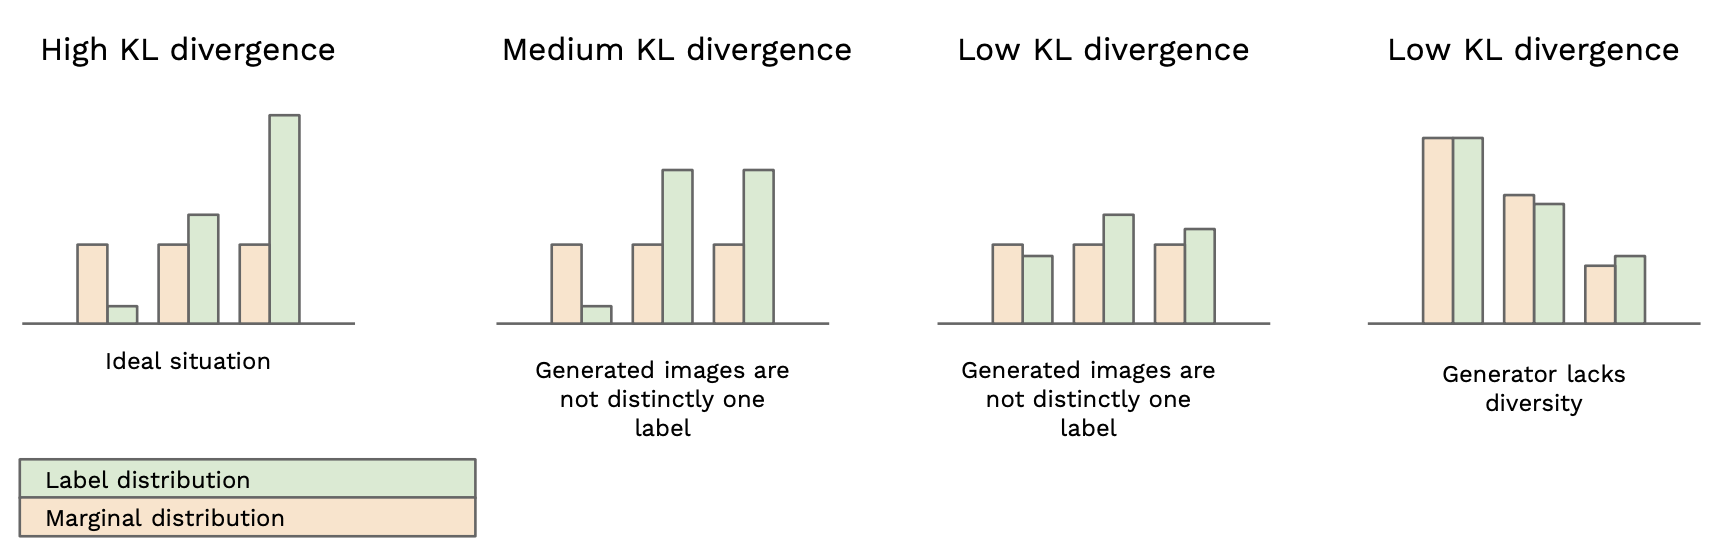
\includegraphics[width=1.0\linewidth]{figs/is_toy}
	\end{figure}
	\myfootnotewithlink{https://medium.com/octavian-ai/a-simple-explanation-of-the-inception-score-372dff6a8c7a}{image credit: https://medium.com/octavian-ai/a-simple-explanation-of-the-inception-score-372dff6a8c7a}
\end{frame}
%=======
\subsection{Inception score}
%=======
\begin{frame}{Evaluation of likelihood-free models}
		\begin{block}{What do we want from samples?}
		\begin{itemize}
			\item Sharpness $\Rightarrow$ low $H(y | \bx) = - \sum_{y} \int_{\bx} p(y, \bx) \log p(y | \bx) d\bx$.
			\item Diversity $\Rightarrow$ high $H(y)  = - \sum_{y} p(y) \log p(y)$.
		\end{itemize}
	\end{block}
	\begin{block}{Inception Score}
		\vspace{-0.3cm}
		\footnotesize
		\begin{align*}
			IS &= \exp(H(y) - H(y | \bx)) \\ 
			&= \exp \left( - \sum_{y} p(y) \log p(y) + \sum_{y} \int_{\bx} p(y, \bx) \log p(y | \bx) d\bx\right) \\
			&= \exp \left( \sum_{y} \int_{\bx} p(y, \bx) \log \frac{p(y | \bx)}{p(y)} d\bx\right) \\ 
			&= \exp \left( \bbE_{\bx} \sum_{y} p(y | \bx) \log \frac{p(y | \bx)}{p(y)} \right) = \exp \left( \bbE_{\bx} KL(p(y | \bx) || p(y)) \right)
		\end{align*}
	\end{block}
	\myfootnotewithlink{https://arxiv.org/abs/1606.03498}{Salimans T. et al. Improved Techniques for Training GANs, 2016}
\end{frame}
%=======
\subsection{Frechet Inception Distance}
%=======
\begin{frame}{Evaluation of likelihood-free models}
	\begin{block}{Theorem (informal)}
		If $\pi(\bx)$ and $p(\bx | \btheta)$ has moment generation functions then
		\vspace{-0.1cm}
		\[
			\pi(\bx) = p(\bx | \btheta) \, \Leftrightarrow \, \bbE_{\pi} \bx^k = \bbE_{p} \bx^k, \quad \forall k \geq 1.
		\]
		\vspace{-0.7cm}
	\end{block}
	This is intractable to calculate all moments.
	\begin{block}{Frechet Inception Distance}
		\vspace{-0.3cm}
		\[
			FID (\pi, p) = \| \mathbf{m}_{\pi} - \mathbf{m}_{p}\|_2^2 + \text{Tr} \left( \bSigma_{\pi} + \bSigma_p - 2 \sqrt{\bSigma_{\pi} \bSigma_p} \right)
		\]
		\vspace{-0.5cm}
	\end{block}
	\begin{itemize}
		\item Representations are the outputs of the intermediate layer from the pretrained classification model.
		\item $\mathbf{m}_{\pi}$, $\bSigma_{\pi} $ are the mean vector and the covariance matrix of feature representations for samples from $\pi(\bx)$
		\item $\mathbf{m}_{p}$, $\bSigma_p$ are the mean vector and the covariance matrix of feature representations for samples from $p(\bx | \btheta)$.
	\end{itemize} 

	\myfootnotewithlink{https://arxiv.org/abs/1706.08500}{Heusel M. et al. GANs Trained by a Two Time-Scale Update Rule Converge to a Local Nash Equilibrium, 2017}
\end{frame}
%=======
\begin{frame}{Evaluation of likelihood-free models}
	\begin{figure}
		\centering
		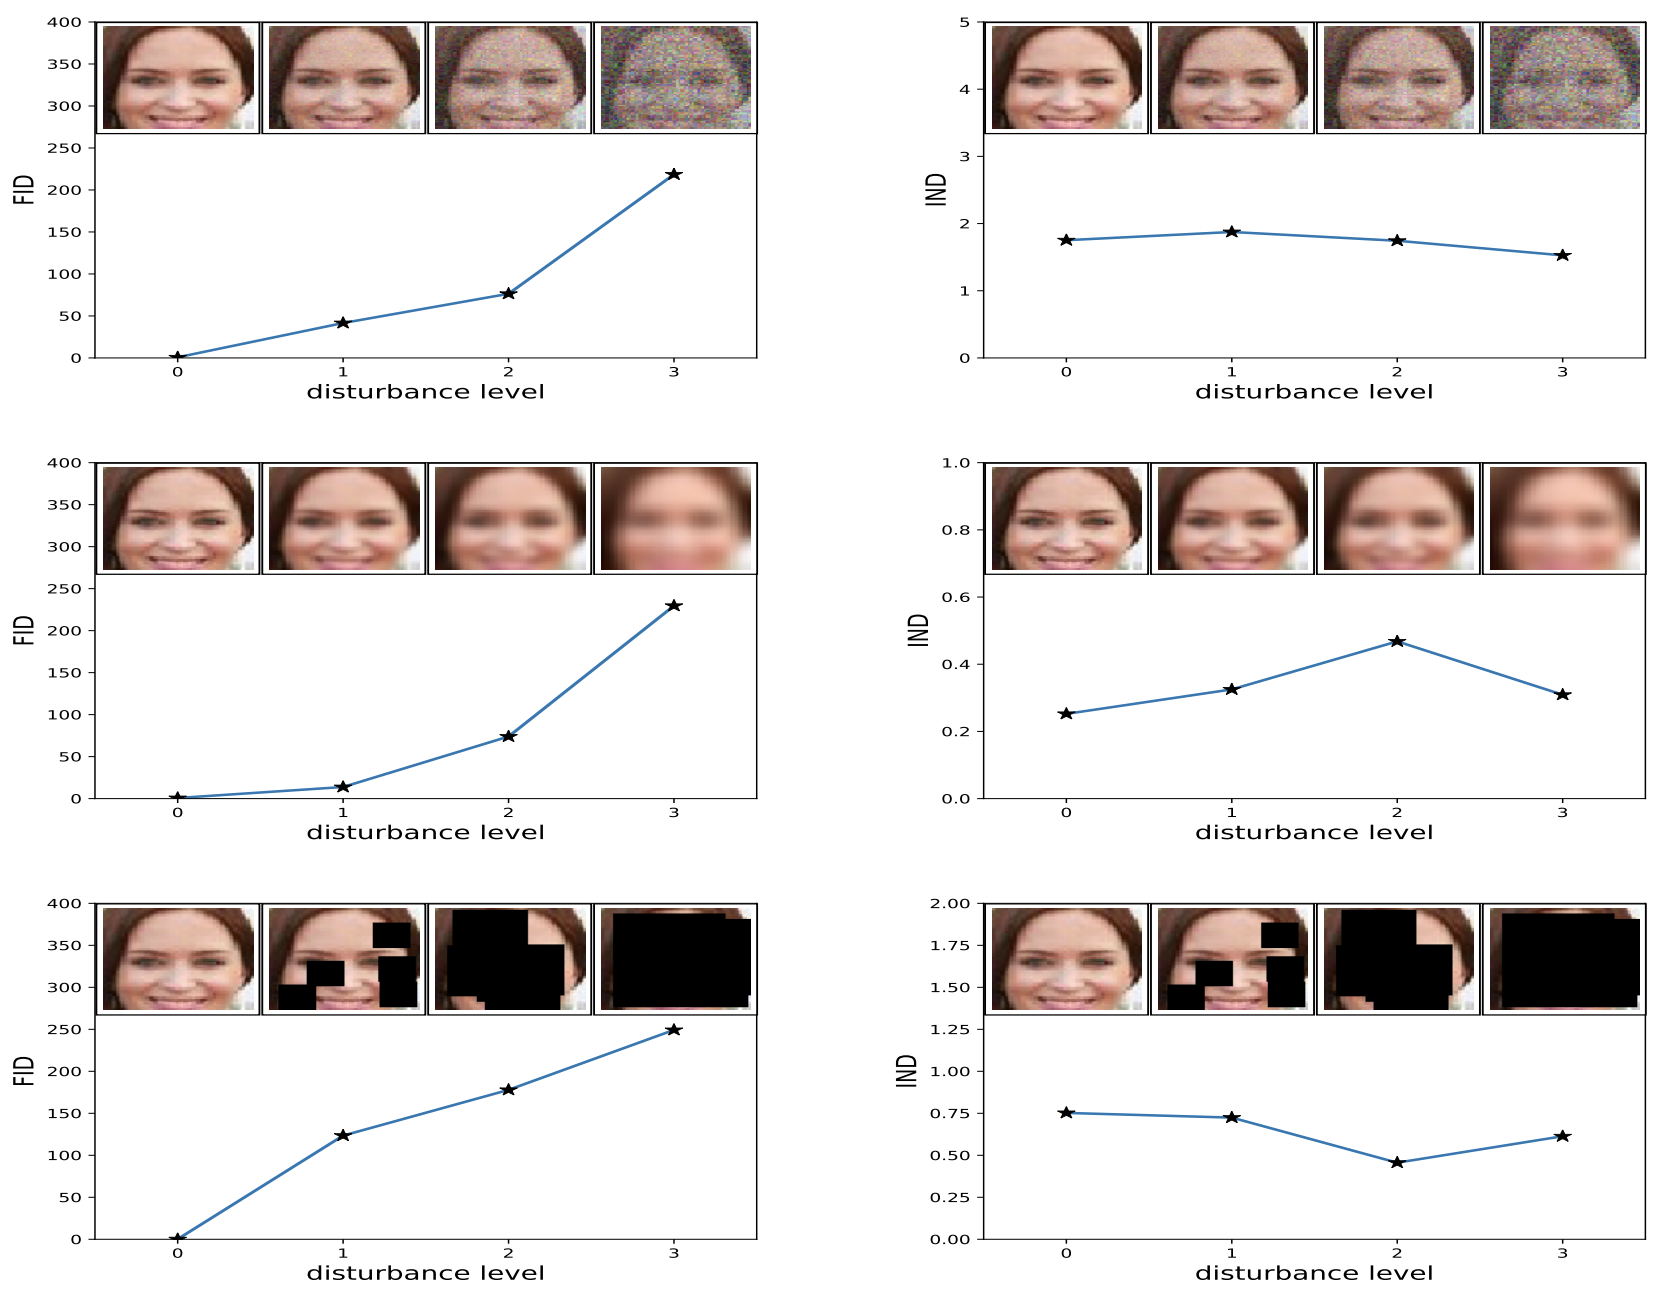
\includegraphics[width=0.9\linewidth]{figs/fid_results}
	\end{figure}
	\myfootnotewithlink{https://arxiv.org/abs/1706.08500}{Heusel M. et al. GANs Trained by a Two Time-Scale Update Rule Converge to a Local Nash Equilibrium, 2017}
\end{frame}
%=======
\begin{frame}{Limitations}
	\vspace{-0.5cm}
	\begin{block}{Inception Score}
		\vspace{-0.5cm}
		\[
			IS =  \exp \left( \bbE_{\bx} KL(p(y | \bx) || p(y)) \right)
		\]
		\vspace{-0.7cm}
	\end{block}
	\begin{itemize}
		\item If generator produces images with a different set of labels from the classifier training set, IS will be low.
		\item If generator produces one image per class, the IS will be perfect (there is no measure of intra-class diversity).
	\end{itemize}
	\begin{block}{Frechet Inception Distance}
		\vspace{-0.4cm}
		\[
			FID = \| \mathbf{m}_{\pi} - \mathbf{m}_{p}\|_2^2 + \text{Tr} \left( \bSigma_{\pi} + \bSigma_p - 2 \sqrt{\bSigma_{\pi} \bSigma_p} \right)
		\]
		\vspace{-0.7cm}
	\end{block}
	\begin{itemize}
		\item Needs a large sample size for evaluation.
		\item Calculation of FID is slow.
		\item Estimates only two sample moments.
	\end{itemize}
	Both scores depend on the pretrained classifier $p(y | \bx)$.

	\myfootnote{\href{https://arxiv.org/abs/1801.01973}{Barratt S., Sharma R. A Note on the Inception Score, 2018} \\
	\href{https://arxiv.org/abs/1706.08500}{Heusel M. et al. GANs Trained by a Two Time-Scale Update Rule Converge to a Local Nash Equilibrium, 2017}}
\end{frame}
%=======
\subsection{Precision-Recall}
%=======
\begin{frame}{Precision-Recall for Generative Models}
	\begin{block}{What do we want from samples}
		\begin{itemize}
			\item \textbf{Sharpness}: generated samples should be of high quality.
			\item \textbf{Diversity}: their variation should match that observed in the training set.
		\end{itemize}
	\end{block}
	\vspace{-0.5cm}
	\begin{figure}
		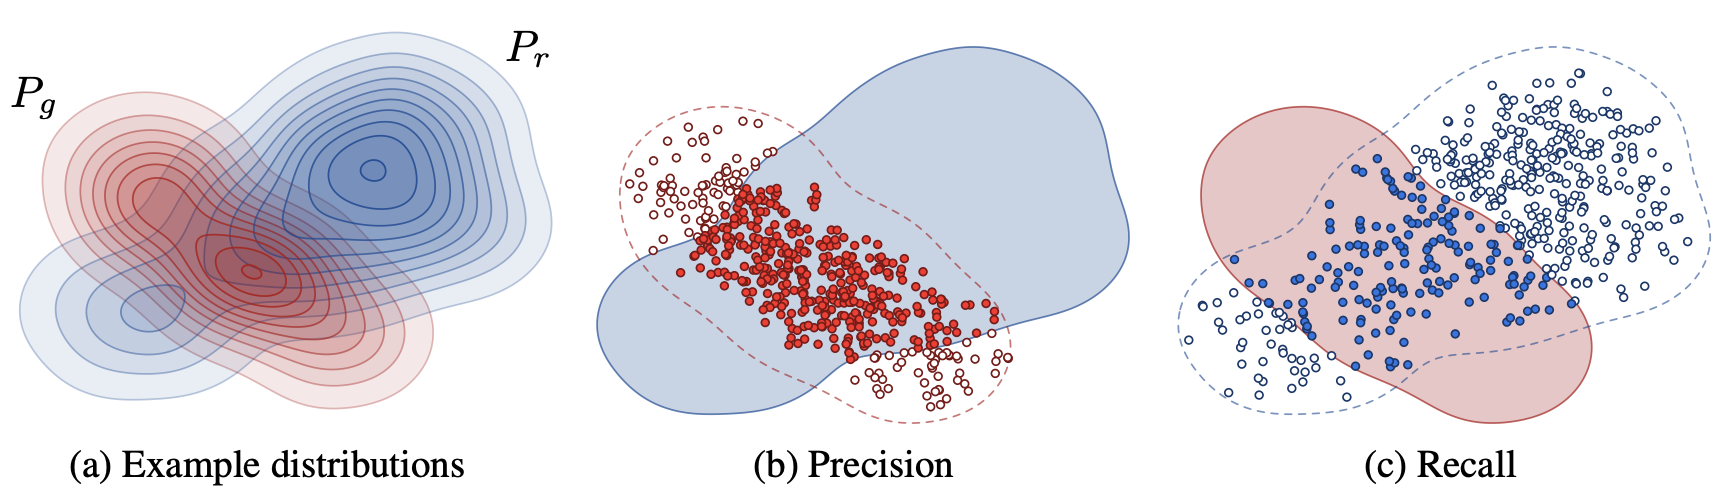
\includegraphics[width=0.95\linewidth]{figs/pr_curve}
	\end{figure}
	\vspace{-0.3cm}
	\begin{itemize}
		\item \textbf{Precision} denotes the fraction of generated images that are realistic.
		\item \textbf{Recall} measures the fraction of the training data manifold covered by the generator.
	\end{itemize}
	\myfootnotewithlink{https://arxiv.org/abs/1904.06991}{Kynkäänniemi T. et al. Improved precision and recall metric for assessing generative models, 2019}
\end{frame}
%=======
\begin{frame}{Precision-Recall for generative models}
	\begin{itemize}
		\item $\cS_{\pi} = \{\bx_i\}_{i=1}^{n} \sim \pi(\bx)$ -- real samples;
		\item $\cS_{p} = \{\bx_i\}_{i=1}^{n} \sim p(\bx | \btheta)$ -- generated samples.
	\end{itemize}
	Embed samples using pretrained classifier network (as previously):
	\[
		\cG_{\pi} = \{\mathbf{g}_i\}_{i=1}^n, \quad \cG_{p} = \{\mathbf{g}_i\}_{i=1}^n.
	\]
	Define binary function:
	\[
		f(\mathbf{g}, \cG) = 
		\begin{cases}
			1, \quad \text{if exists } \mathbf{g}' \in \cG: \| \mathbf{g}  - \mathbf{g}'\|_2 \leq \| \mathbf{g}' - \text{NN}_k(\mathbf{g}', \cG)\|_2; \\
			0, \quad \text{otherwise.}
		\end{cases}
	\]
	\[
		\text{Precision} (\cG_{\pi}, \cG_{p}) = \frac{1}{n} \sum_{\mathbf{g} \in \cG_{p}} f(\mathbf{g}, \cG_{\pi}); \,\, \text{Recall} (\cG_{\pi}, \cG_{p}) = \frac{1}{n} \sum_{\mathbf{g} \in \cG_{\pi}} f(\mathbf{g}, \cG_{p}).
	\]
	\vspace{-0.4cm}
	\begin{figure}
		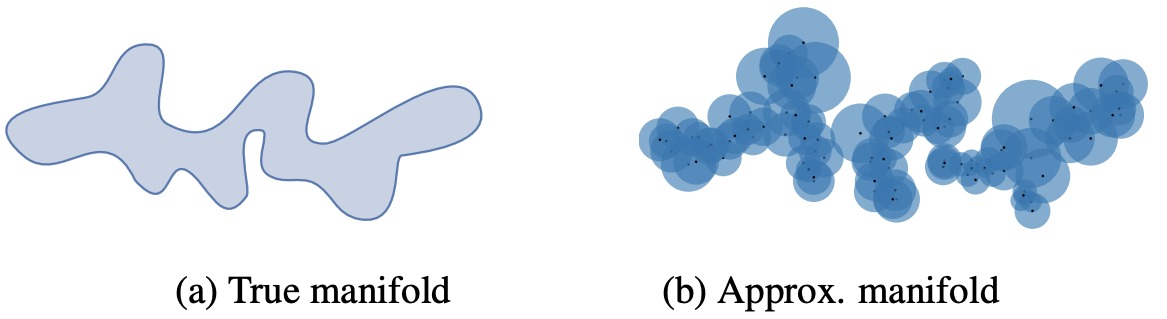
\includegraphics[width=0.7\linewidth]{figs/pr_k_nearest}
	\end{figure}
	\myfootnotewithlink{https://arxiv.org/abs/1904.06991}{Kynkäänniemi T. et al. Improved precision and recall metric for assessing generative models, 2019}
\end{frame}
%=======
\begin{frame}{Precision-Recall for generative models}
	\begin{figure}
		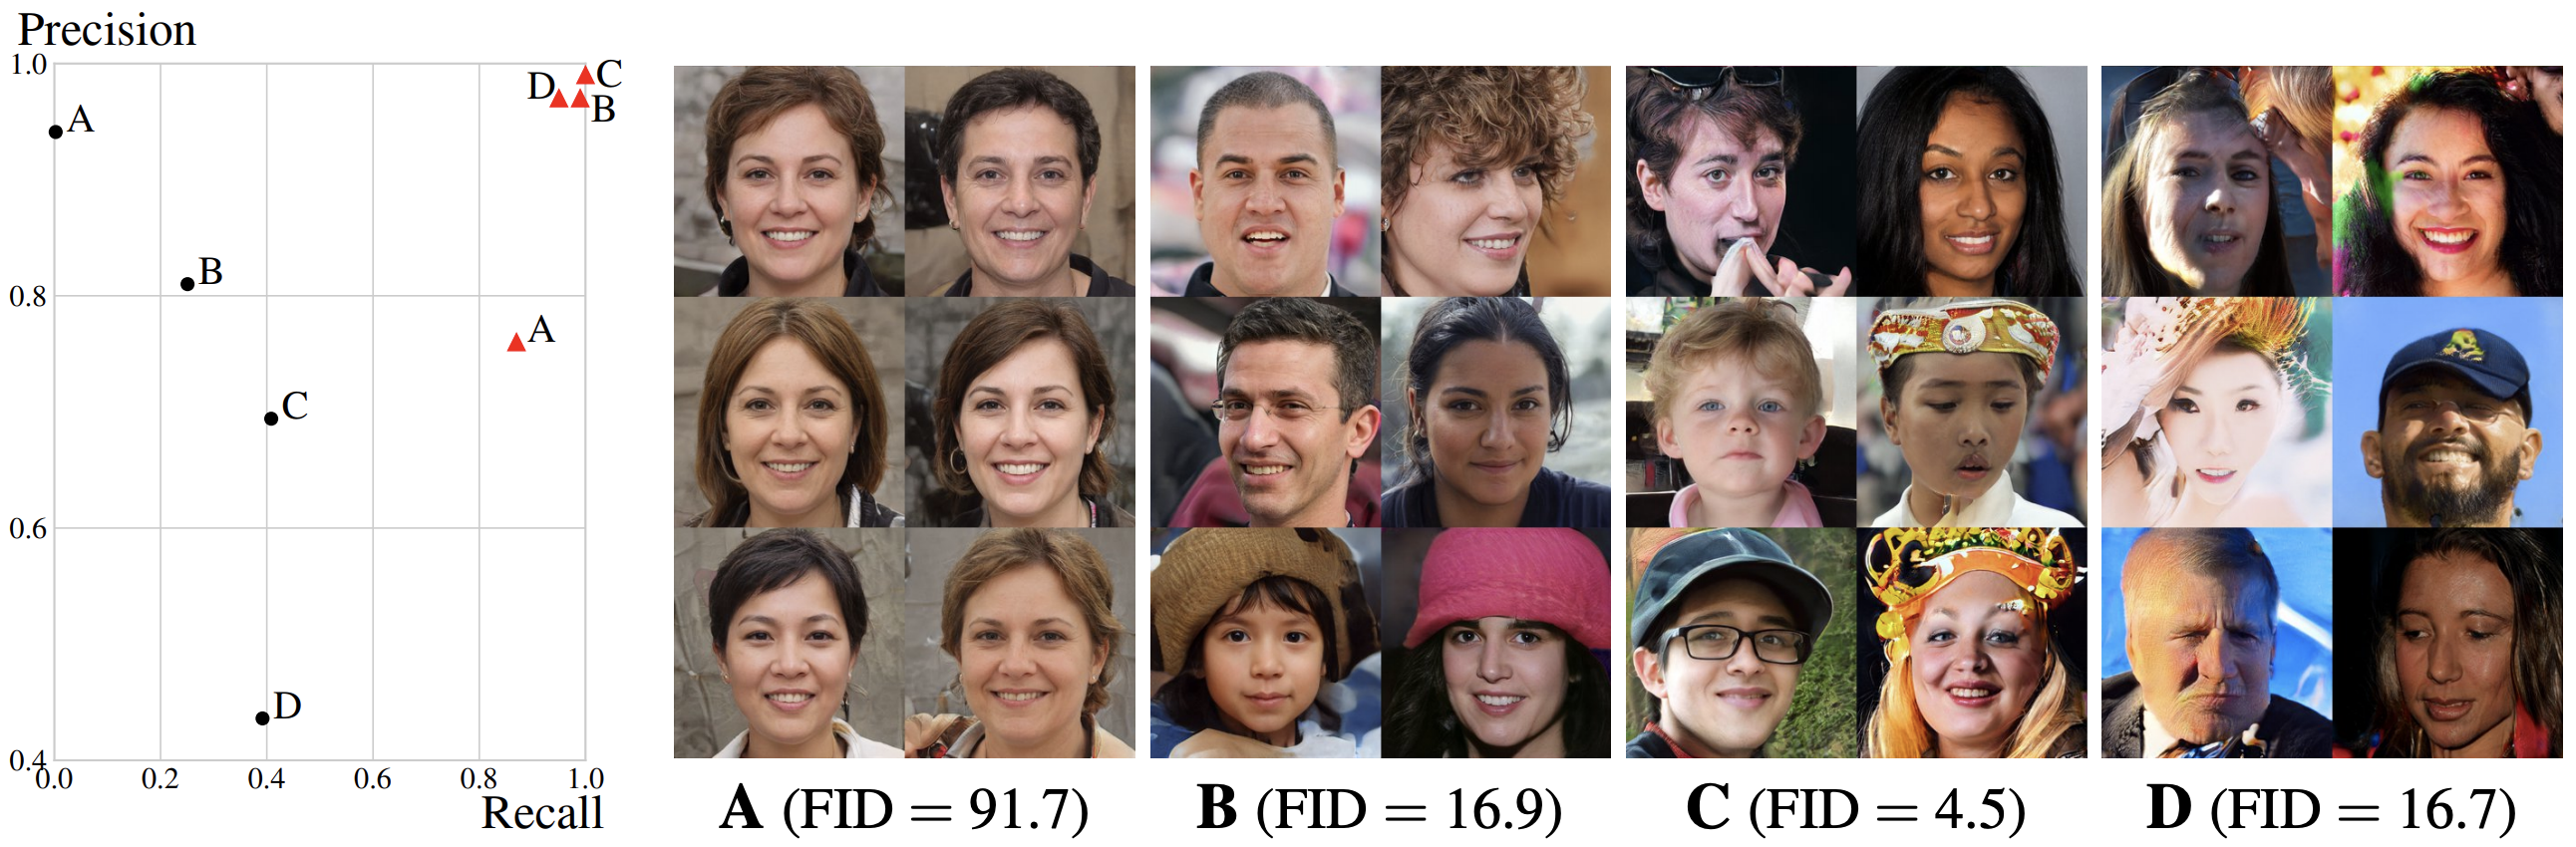
\includegraphics[width=\linewidth]{figs/pr_vs_fid}
	\end{figure}
	\begin{figure}
		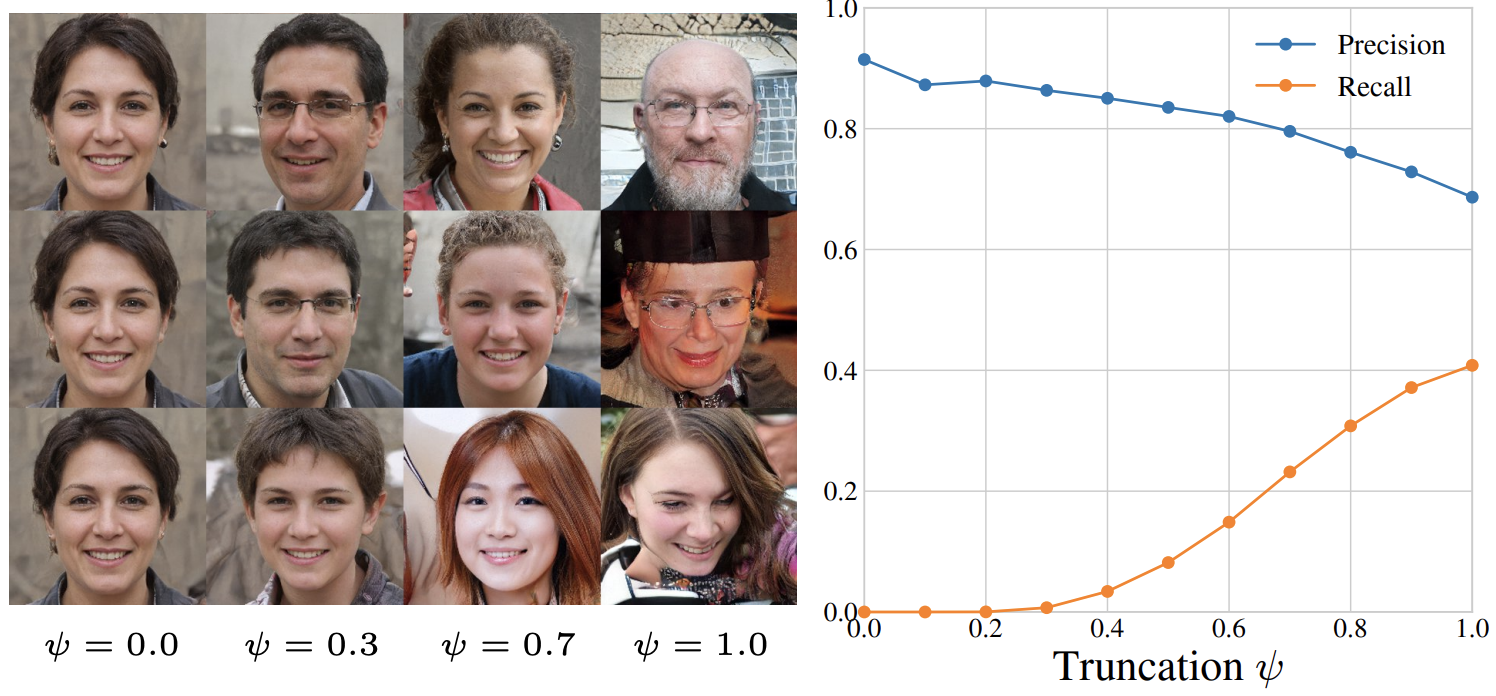
\includegraphics[width=0.75\linewidth]{figs/pr_truncation}
	\end{figure}
	\myfootnotewithlink{https://arxiv.org/abs/1904.06991}{Kynkäänniemi T. et al. Improved precision and recall metric for assessing generative models, 2019}
\end{frame}
%=======
\begin{frame}{Truncation trick}
	\begin{block}{BigGAN: truncated normal sampling}
		\vspace{-0.3cm}
		\[
			p(\bz | \psi) = \cN(\bz | 0, 1) / \int_{-\infty}^\psi \cN(\bz | 0, 1) d\bz
		\]
		Components of $\bz \sim \cN(0, \bI)$ which fall outside a predefined range are resampled.
	\end{block}
	
	\begin{block}{StyleGAN}
		\vspace{-0.2cm}
		\[
			\bz' = \hat{\bz} + \psi \cdot (\bz - \hat{\bz}), \quad \hat{\bz} = \bbE_{\bz} \bz
		\]
		\vspace{-0.2cm}
		\begin{itemize}
			\item Constant $\psi$ is a tradeoff between diversity and fidelity. 
			\item $\psi=0.7$ is used for most of the results.
		\end{itemize}
	\end{block}

	\myfootnote{\href{https://arxiv.org/abs/1809.11096}{Brock A., Donahue J., Simonyan K. Large Scale GAN Training for High Fidelity Natural Image Synthesis, 2018} \\
	\href{https://arxiv.org/abs/1812.04948}{Karras T., Laine S., Aila T. A Style-Based Generator Architecture for Generative Adversarial Networks, 2018}}
\end{frame}
%=======
\begin{frame}{Summary}
	\begin{itemize} 
		\item f-divergence family is a unified framework for divergence minimization, which uses variational approximation. Standard GAN is a special case of it.
		\vfill
		\item We need measure of quality for implicit models like GANs. One way is to analyze sharpness and diversity of samples.
		\vfill 
		\item Inception Score and Frechet Inception Distance are the common metrics for GAN evaluation, but both of them have drawbacks.
		\vfill
		\item Precision-recall allows to select model that compromises the sample quality and the sample diversity.	
		\vfill 
		\item Truncation tricks help to select model with compomised samples: diverse and sharp.
	\end{itemize}
\end{frame}
%=======
\end{document} 